\documentclass[slovene,11pt,a4paper]{article}
%\usepackage{fullpage}
\usepackage[margin=2cm]{geometry}

\usepackage[T1]{fontenc}



%dodatni paketki:
\usepackage{graphicx}
\usepackage{amsmath,amsfonts,amsthm} %matematicni paket
\usepackage{color} % omogoča barvno pisanje
\usepackage[utf8]
{inputenc}
\usepackage[slovene]{babel} % slovenski jezik/hyphenation
\usepackage{hyperref} %naredi vse povezave rečerenc, kazala,...
\numberwithin{equation}{section} % Number equations within sections (i.e. 1.1, 1.2, 2.1, 2.2 instead of 1, 2, 3, 4)
\numberwithin{figure}{section} % Number figures within sections (i.e. 1.1, 1.2, 2.1, 2.2 instead of 1, 2, 3, 4)
\numberwithin{table}{section} % Number tables within sections (i.e. 1.1, 1.2, 2.1, 2.2 instead of 1, 2, 3, 4)
\usepackage{eurosym} %za znak €

\usepackage{mathrsfs}
\usepackage{mathabx} % za kemisjke smeri in naslednje 3 vstrice
\catcode`_=12
\begingroup\lccode`~=`_\lowercase{\endgroup\let~\sb}
\mathcode`_="8000


\usepackage[margin=2cm]{geometry}



\begin{document}
\begin{titlepage}

\newcommand{\HRule}{\rule{\linewidth}{0.5mm}} % Defines a new command for the horizontal lines, change thickness here

\center % Center everything on the page

%----------------------------------------------------------------------------------------
%	LOGO
%----------------------------------------------------------------------------------------

%\includegraphics{Logo}\\[1cm] % Include a department/university logo - this will require the graphicx package
 
%----------------------------------------------------------------------------------------


\includegraphics[width=2cm]{slike/aaa}\\[0.5cm]
 
%----------------------------------------------------------------------------------------
%	NASLOV DELA
%----------------------------------------------------------------------------------------
\textit{Univerza v Ljubljani}\\
\textit{Fakulteta za {\color{red}matematiko in fiziko}}\\[0.5cm]

\emph{Oddelek za fiziko}\\[0.5cm] % Oddelek za fiziko


%----------------------------------------------------------------------------------------
%	TITLE SECTION
%--------------------------------------------------------------------------------------
\HRule \\[0.4cm]
\huge {\bfseries 11. naloga: - Stohastični populacijski model}\\[0.4cm] % NASLOV SEMINARJA
\HRule \\[0.5cm] 

 \textsc{\large Poročilo pri predmetu modelska analiza 1}\\
 \textsc{\large 2015/2016}\\[1cm] % SEMINASKO DELO
 
%----------------------------------------------------------------------------------------
%	AUTHOR SECTION
%----------------------------------------------------------------------------------------



% If you don't want a supervisor, uncomment the two lines below and remove the section above
\Large \emph{Avtor:}\\
Klemen \textsc{Rahne}\\
28152028\\[2cm]
%----------------------------------------------------------------------------------------
%	DATUM
%----------------------------------------------------------------------------------------

{\large \today } \\[0.5cm] % Date, change the \today to a set date if you want to be precise

	

\end{titlepage}


%----------------------------------------------------------------------------------------
%	KAZALO
%----------------------------------------------------------------------------------------

%\tableofcontents

%----------------------------------------------------------------------------------------
%	ZAČETEK TEKSTA
%----------------------------------------------------------------------------------------


\section{Porazdelitev izumrlih časov}

Obravnavajmo model populacije. Analitično spreminjanje populacije zapišemo:
\begin{equation}
\frac{d N}{dt}= N (\beta_r - \beta_s )
\end{equation}
kjer je $N$ število populacije, ter $\beta_s$, $\beta_r$ koeficienta umrljivosti, rojstva populacije. Rešitev enačbe je eksponentno naraščanje/padanje populacije. Pri stohastični modelu spreminjamo populacijo po naključnem številu, ki je porazdeljen po nekem zakonu. Iz zgornje enačbe lahko zapišemo:
\begin{equation}
\Delta N= N (\beta_r - \beta_s ) \Delta t
\label{enačba-1}
\end{equation}
Spreminjanje populacije je porazdeljeno po Poissonovi porazdelitvi, s povprečno vrednostjo $\overline{ N}= N \beta \Delta t$. Torej v vsakem koraku k trenutni populaciji prištejemo spremembo populacije:
\begin{equation}
N_{i+1}=N_i - \mathcal{P}(N_i \beta \Delta t)
\label{enačba-2}
\end{equation}

\begin{figure}[h]
\centering
\begin{minipage}{0.5\textwidth}
\centering
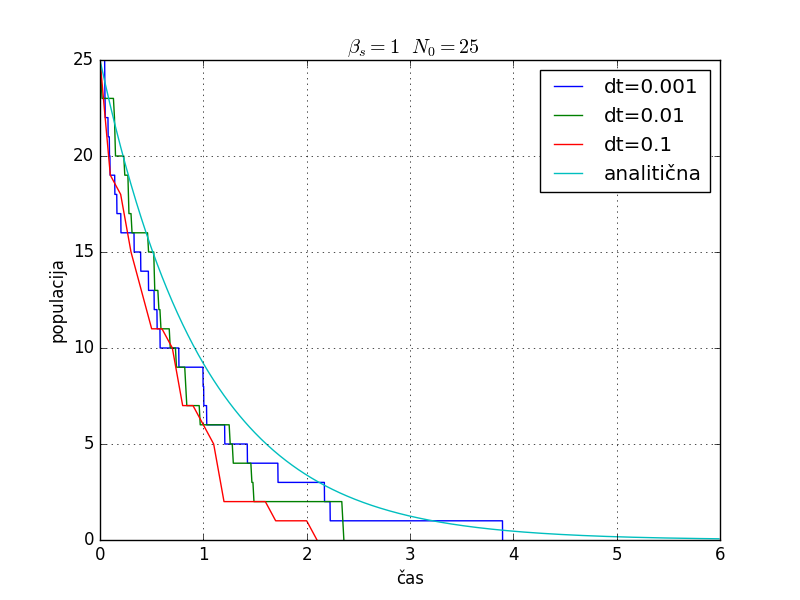
\includegraphics[scale=0.45]{slike/populacija_umiranje_preprosto_25.png}
%\caption{first figure}
\end{minipage}\hfill
\begin{minipage}{0.5\textwidth}
\centering
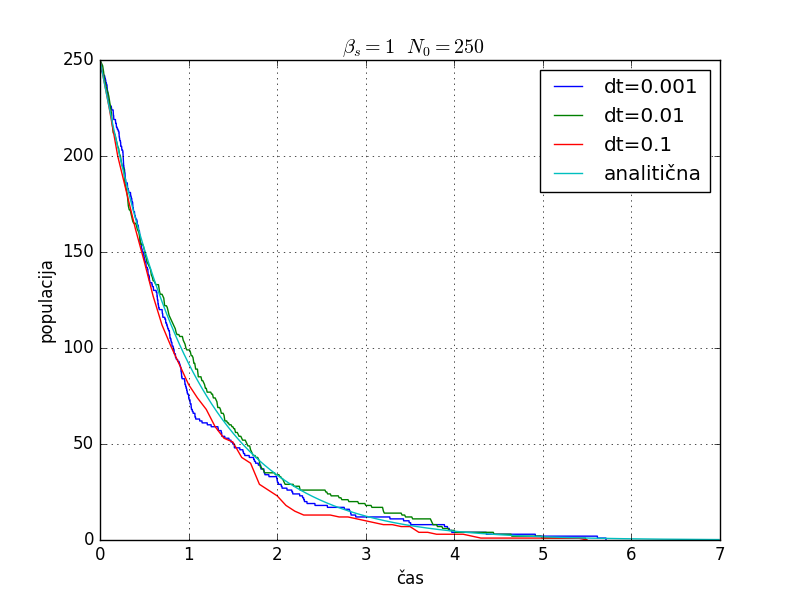
\includegraphics[scale=0.45]{slike/populacija_umiranje_preprosto_250.png}
%\caption{second figure}
\end{minipage}
\begin{minipage}{0.5\textwidth}
\centering
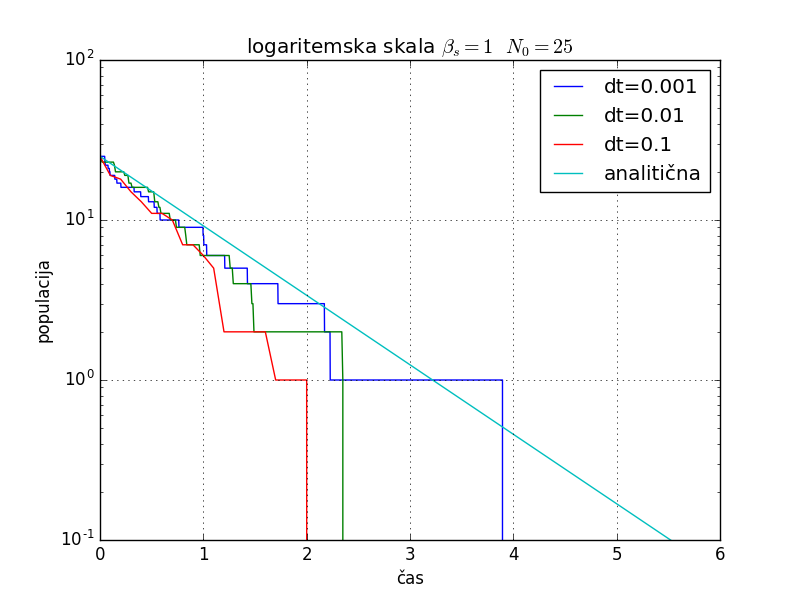
\includegraphics[scale=0.45]{slike/populacija_umiranje_preprosto_25_log.png}
%\caption{first figure}
\end{minipage}\hfill
\begin{minipage}{0.5\textwidth}
\centering
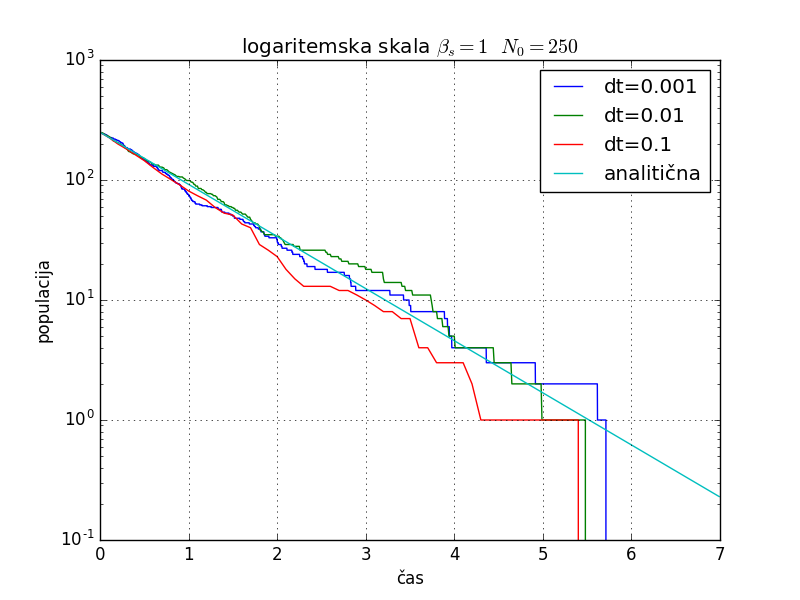
\includegraphics[scale=0.45]{slike/populacija_umiranje_preprosto_250_log.png}
%\caption{second figure}
\end{minipage}
\caption{Primerjava reštev populacijskih modelov. Spodnja slika je enaka zgornji slike, le da je $y$ ordinata v logaritemski skali. Na levi strani imamo začetno populacijo $25$, na desni $250$. Opazimo, da se pri večji začetni populaciji stohastično dobljene spremembe populacije bolje prilagajajo analitični rešitvi. Prav tako opazimo, da se manjši časovni intervali bolje prilagajajo analitični rešitvi. }
\end{figure}

Kot posledica stohastične obravnave naše populacije, pride število naše  populacije na nič. Takrat naša populacija umre, saj v njej ni več oseb. V primerjavi z analitično rešitvijo (pri kateri se vrednost populacije priblišuje priti 0) pridemo sedaj do novega podatka v našem modelu-izumrlem času. Zaradi stohastičnega modela naše populacije dobimo pri vsaki generaciji populacijskega modela do drugačnega časa izumrtja. Zato si oglejmo porazdelitve teh časov.



\begin{figure}[h]
\centering
\begin{minipage}{0.5\textwidth}
\centering
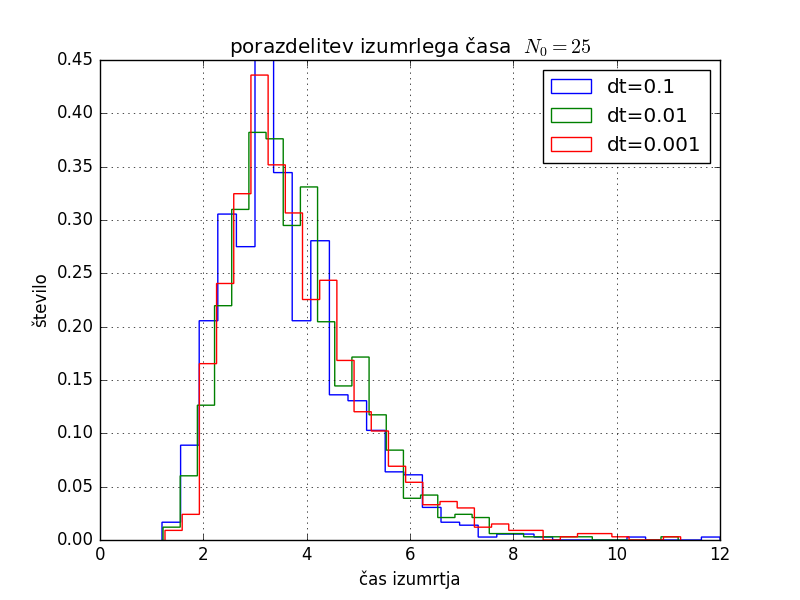
\includegraphics[scale=0.45]{slike/porazdelitev_umrlicas_25.png}
%\caption{first figure}
\end{minipage}\hfill
\begin{minipage}{0.5\textwidth}
\centering
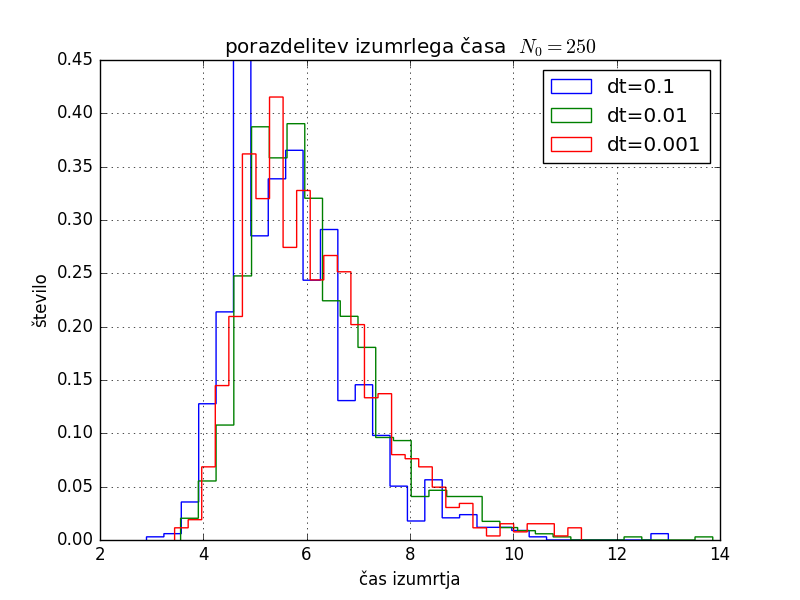
\includegraphics[scale=0.45]{slike/porazdelitev_umrlicas_250.png}
%\caption{second figure}
\end{minipage}

\caption{Porazdelitve časa izurmtja za populaciji z različnima začetnima populacijama (levo $N_0=25$, desno $N_0=250$). Opazimo, da v posameznem modelu porazdelitve bistveno ne odstopaje med seboj z različnimi diferencialnimi časi ($dt$). Porazdelitev ima pri obeh populacijah en izrazit vrh, ki pa se razlikujeta v položaju med populacijema (pri $N_0=25$ pri okoli $3.5$, pri $N_0=250$, pa okoli $5$). To je povsem pričakovano, saj za izumrtje večje populacije pri enakem koeficientu umrljivosti potrebno več časa. Pri vsaki populaciji sem generiral $1000$ razpradnih časov. Histogrami se normalizirani.}
\end{figure}

\subsection{Umrljivost z rodnostjo}

Do sedaj smo v našem populacijskem modelu upoštevali le smrtnost. Po enačbi \ref{enačba-2} sedaj generirajmo spremembo populacije, tako da upoštevamo še rojstvo:

\begin{equation}
N_{i+1}=N_i - \mathcal{P}(N_i \beta_s \Delta t) + \mathcal{P}(N_i \beta_r \Delta t)
\label{enačba-3}
\end{equation}
Analitično je rešitev exponentna funkcija, s parametrom $\beta$ v eksponentu, ki je razlika koeficienta rojstva in umrljivosti. Posledično je ponovno analitična rešitev eksponentno padanje/naraščanje populacije.



\begin{figure}[h]
\centering
\begin{minipage}{0.5\textwidth}
\centering
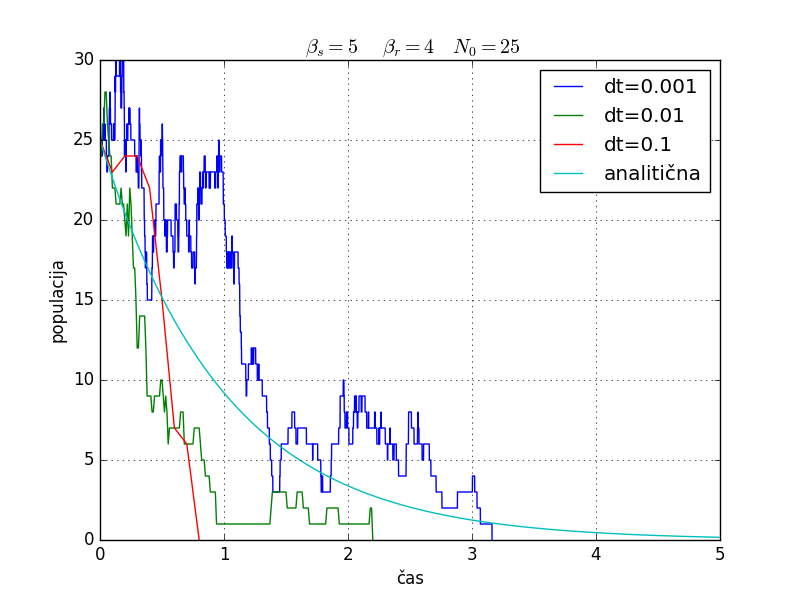
\includegraphics[scale=0.45]{slike/populacija_umiranje_rojstvo_preprosto_25.png}
%\caption{first figure}
\end{minipage}\hfill
\begin{minipage}{0.5\textwidth}
\centering
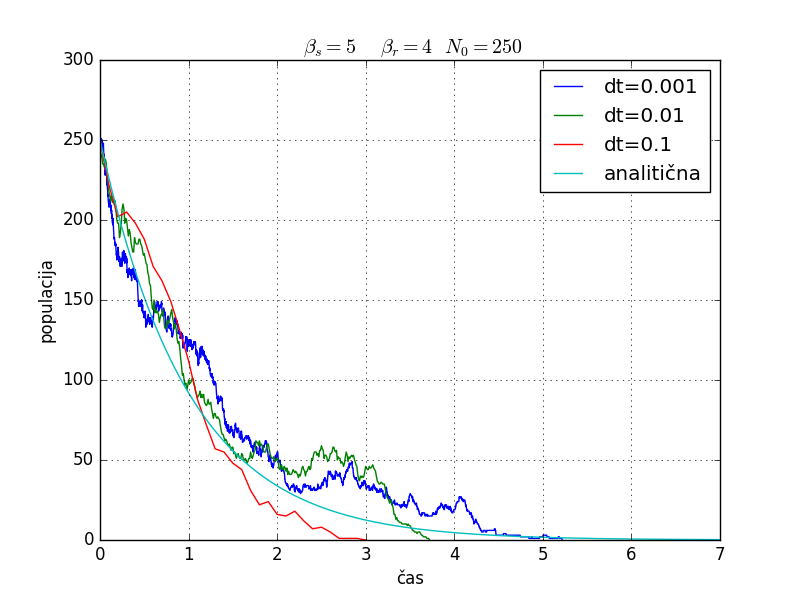
\includegraphics[scale=0.45]{slike/populacija_umiranje_rojstvo_preprosto_250.png}
%\caption{second figure}
\end{minipage}
\caption{Primerjava populacijskih modelov. Na levi strani imamo modele z začetno populacijo $N_0=25$, na desni z $N_0=250$. Sklepamo, da model z začetno vrednostjo populacije $N_0=250$ lešpše sledi analitični rešitvi.}
\end{figure}



\begin{figure}[h]
\centering
\begin{minipage}{0.5\textwidth}
\centering
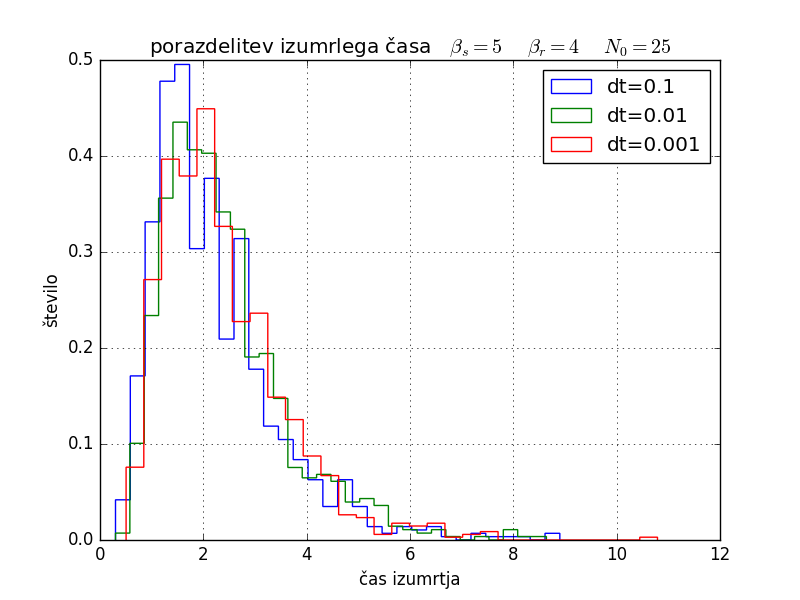
\includegraphics[scale=0.45]{slike/porazdelitev_umrlirojstvocas_25.png}
%\caption{first figure}
\end{minipage}\hfill
\begin{minipage}{0.5\textwidth}
\centering
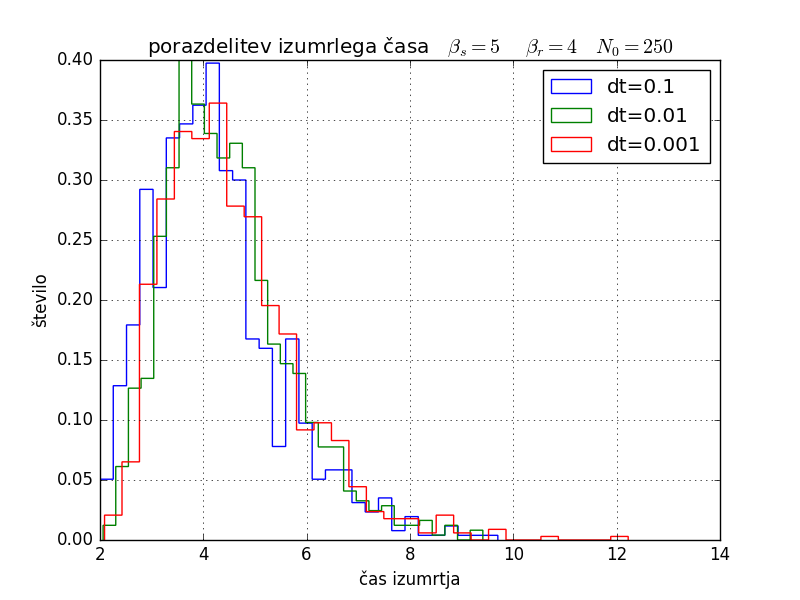
\includegraphics[scale=0.45]{slike/porazdelitev_umrlirojstvocas_250.png}
%\caption{second figure}
\end{minipage}
\caption{Primerjava porazdelitev časov izumrtja. Ponovno ima porazdelitev vrh, pri začetni populacije $N_0=25$ je okoli $2$, pri $N_0=250$ je okoli 4. Opazimo, da so porazdelitve pri modelih z enako začetno vrednostjo skoraj enake. Histogram je normaliziran, za vsako porazdelitev je bilo generiranih $1000$ časov izumrtja.}
\end{figure}



\begin{figure}[h]
\centering
\begin{minipage}{0.5\textwidth}
\centering
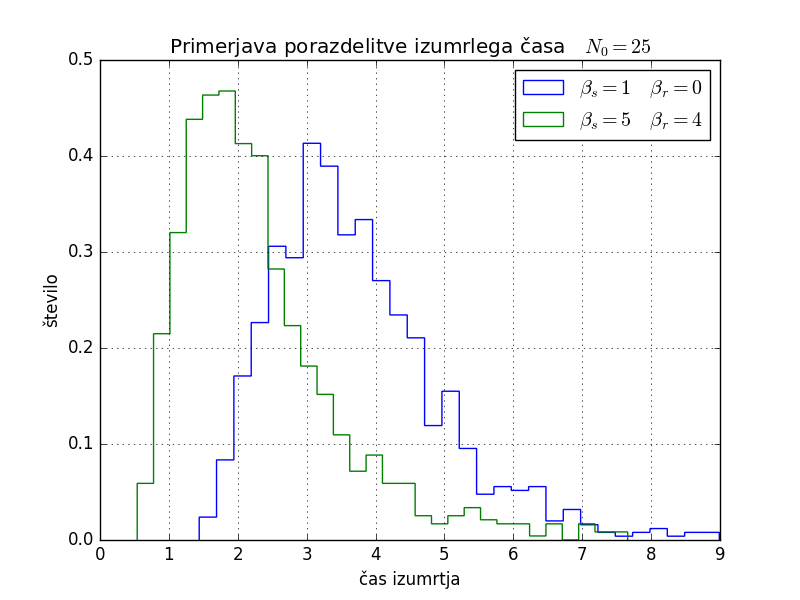
\includegraphics[scale=0.45]{slike/porazdelitev_preprost_umrlirojstvocas_25.png}
%\caption{first figure}
\end{minipage}\hfill
\begin{minipage}{0.5\textwidth}
\centering
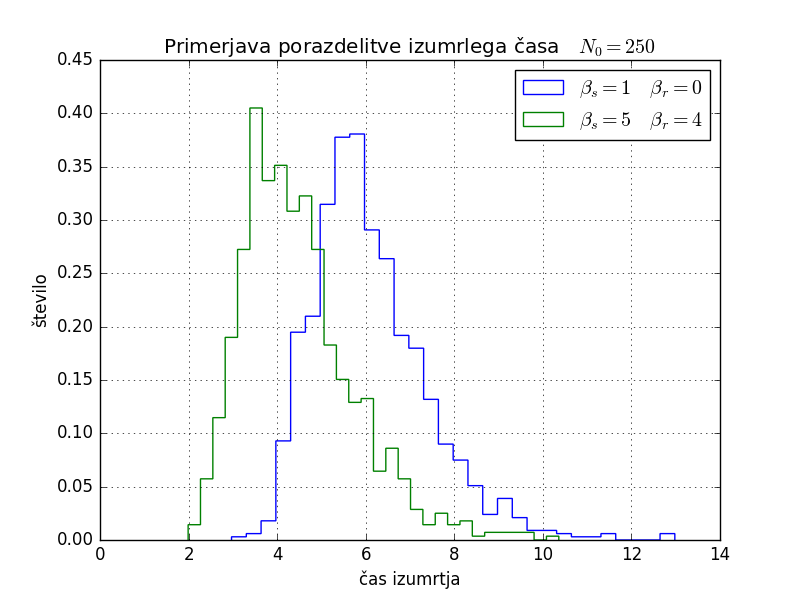
\includegraphics[scale=0.45]{slike/porazdelitev_preprost_umrlirojstvocas_250.png}
%\caption{second figure}
\end{minipage}
\caption{Primerjava porazdelitev časov izumrtja. Na levi je model z začetno populacijo $N_0=25$, na desni model z začetno populacijo $N_0=250$. V vseh primerih je časovna diferenca $0.01$. V obeh  populacijah opazimo, da z vpeljavo rodnosti se vrh porazdelitve pomakne levo (zmanjša čas izumrtja). }
\end{figure}

\clearpage

\section{Matrika prehodov}
Spreminjanje populacije lahko zapišemo tudi s pomočjo matrike, s pomočjo katere napovemo verjetnostne prehode iz trenutnega stanja v naslednje stanje:
\begin{equation}
x_{i+1}=Mx_i
\end{equation}
kjer je $x$ vektor populacije in $M$ prehodna matrika. V vektorju populacije se skrivajo verjetnosti oz. delež populacije v stanju s številom populacije s pripadajočim indeksom. Primer: $x=(0,0.25,0.75,0)$, pomeni, da je verjetnost, da ima sistem $1$ osebo enako $25\%$ in $2$ osebi $75\%$.
V matriko $M$ na mesto $ij$ zapišemo verjetnost za prehod števila populacije iz stanja $i$ v stanje $j$. Spremembe števila populacije so porazdeljene po Poissonovi porazdelitvi. V našem primeru bomo naredili dve poenostavitvi: $1)$ Stanje sistema se lahko spremeni le za ena; $2)$ verjetnost za preho bo majhna in enaka $r_i=n_i \beta	dt$, kjer je $n_i$ število populacije v stanju $i$ (je enako $i$), $\beta$ konstanta umrljivosti/rojstva, ter $dt$ diferencial časa. Torej ima naša matrika na diaginalah vrednosti $1-r_s-r_r$, nad diagonalo $r_s$, pod diagonalo $r_r$.

\begin{figure}[h]
\begin{center}
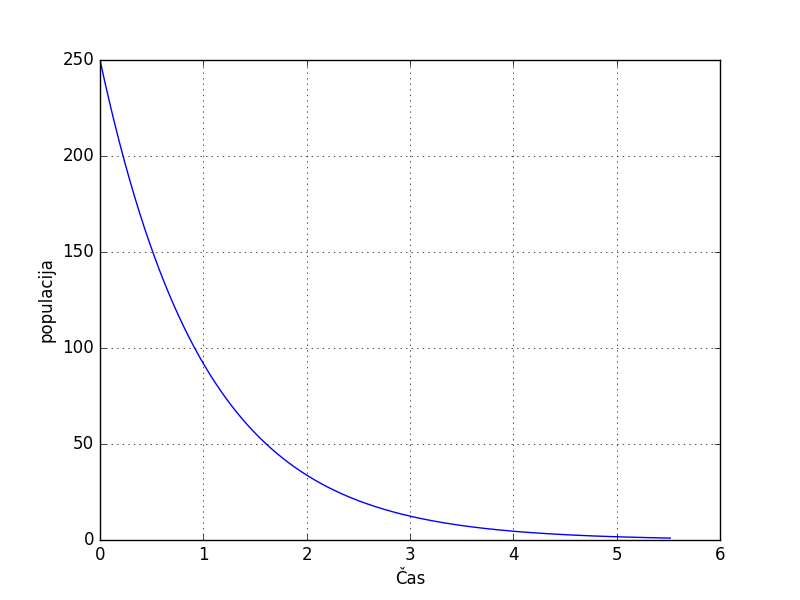
\includegraphics[scale=0.65]{slike/populacija_matrika_beta_0.png}
\caption{Ćasovni potek spreminjanje populacije s uporabo matrike prehodov. Začetno število populacije je $250$, na vrednost pod $0$ pade v času $5.5129$. Analitična rešitev zavzame povsem enako obliko. Prav tako enako obliko zavzame, če upoštevamo samo smrtnost ($\beta=1$) ali smrtnost in rojstvo ($\beta_r=4, \beta_s=5$).}
\label{graf-enak-za vse}
\end{center}
\end{figure}


\begin{figure}[h]
\begin{center}
\begin{minipage}{\textwidth}
\centering
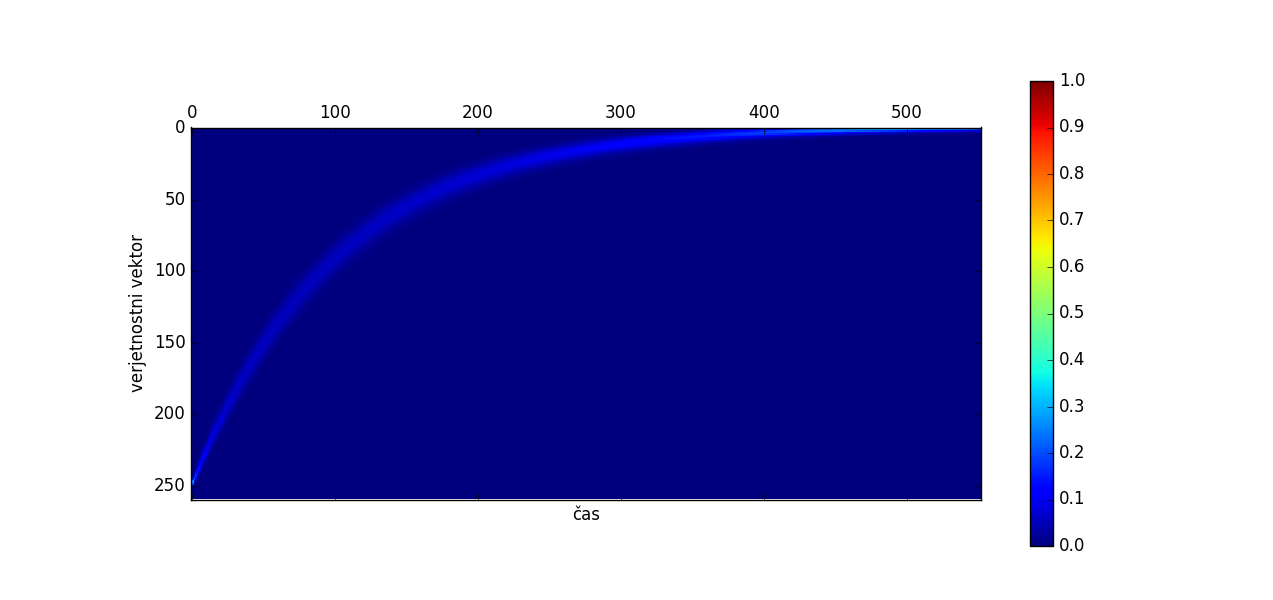
\includegraphics[scale=0.6]{slike/matrika_porazdelitve_beta_0.png}
%\caption{first figure}
\end{minipage}\hfill
\end{center}
\caption{Kako se spreminja verjetnost, da je v danem stanju sistem.}
\end{figure}



\begin{figure}[h]
\centering
\begin{minipage}{0.5\textwidth}
\centering
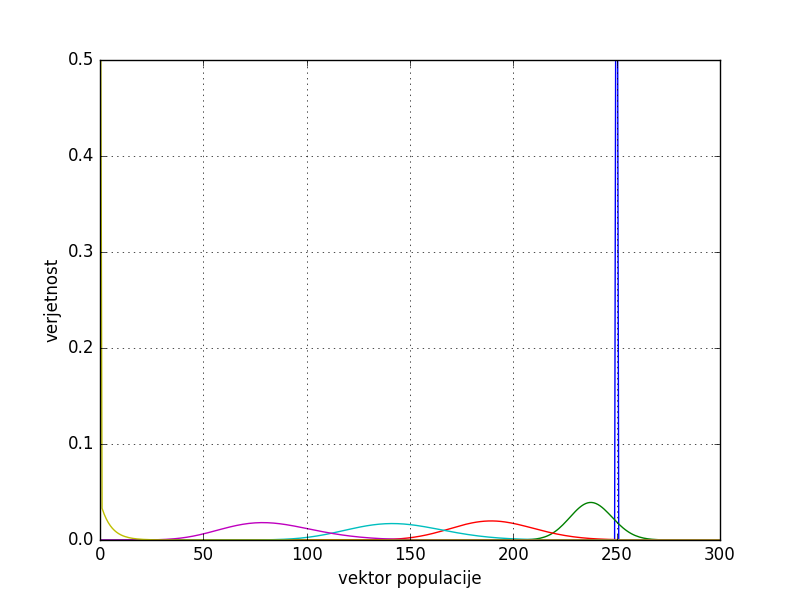
\includegraphics[scale=0.45]{slike/smrtnost_rodnost_disperzija.png}
%\caption{first figure}
\end{minipage}\hfill
\begin{minipage}{0.5\textwidth}
\centering
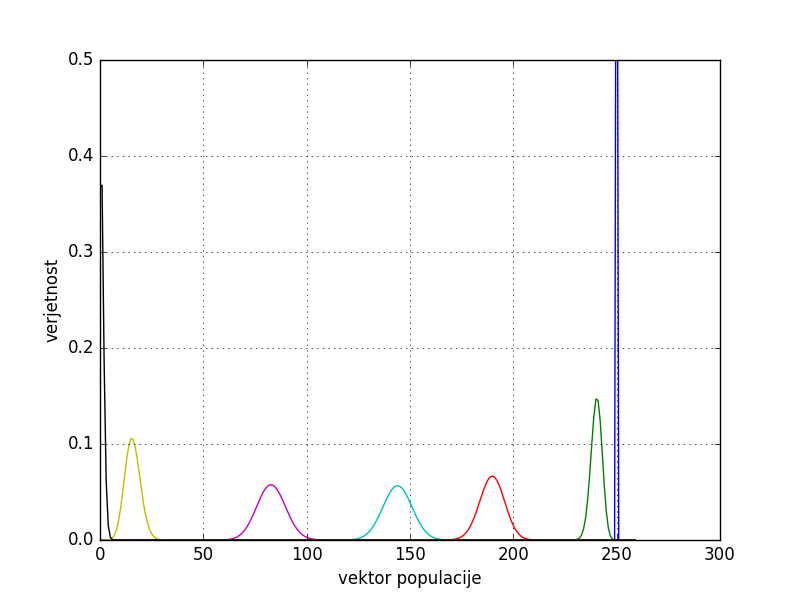
\includegraphics[scale=0.45]{slike/test.png}
%\caption{second figure}
\end{minipage}
\caption{Primerjava, kako se širina verjetnostnega vektorja spreminja s časom. Na začetku imamo $\delta$ funkcijo pri $250$, nato se zelo hitro približa gaussovi funkciji. Oblika se ohranja, dokler se skupna populacija ne približa $0$. Tam se preoblikuje v $\delta$ fukcijo pri $0$. Na levi strani je uporabljena samo umrljivost($\beta_=1$), medtem ko je na desni uporabljena še rodnost ($\beta_s=5, \beta_r=4$). Na desni strani se na zašetku (zelena krivulja) opazi še verjetnost, ki presega začetno vrednost populacije. To je posledica vpeljave rodnosti, vendar to na popvprečno/pričakovano vrednost nima vpliva-glej \ref{graf-enak-za vse}. Diferencial časa na levi je bil $0.001$, na desni pa $0.0001$.}
\end{figure}

\clearpage
\section{Lisice in zajci}
Imamo model zajcev in lisic:
\begin{equation}
\begin{aligned}
\dot{Z}=&\alpha Z-\beta Z L \\
\dot{L} =& - \gamma L+\delta Z L
\end{aligned}
\end{equation}
Podobno kot v prvem delu te naloge računamo novo populacijo s pomočjo naključnih števil, ki so porazdeljeni po Poissonovi porazdelitvi:

\begin{equation}
\begin{aligned}
Z_{i+1}=&Z_i + \mathcal{P}(Z_i \alpha \Delta t) - \mathcal{P}(Z_i L_i \beta \Delta t) \\
L_{i+1}=&L_i + \mathcal{P}(L_i \gamma \Delta t) - \mathcal{P}(Z_i L_i \delta \Delta t)
\end{aligned}
\label{zajci-lisice-1}
\end{equation}

\begin{figure}[h]
\centering
\begin{minipage}{0.5\textwidth}
\centering
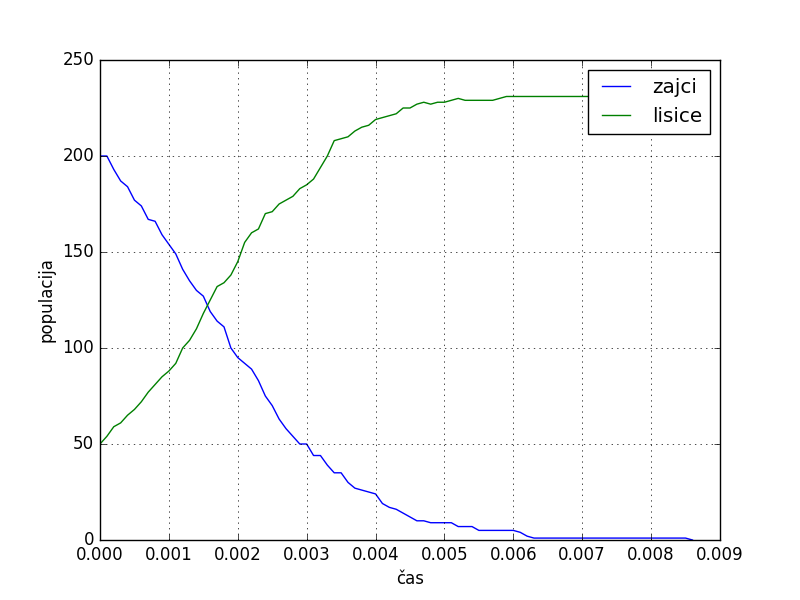
\includegraphics[scale=0.45]{slike/zajci_lisice_populacija.png}
%\caption{first figure}
\end{minipage}\hfill
\begin{minipage}{0.5\textwidth}
\centering
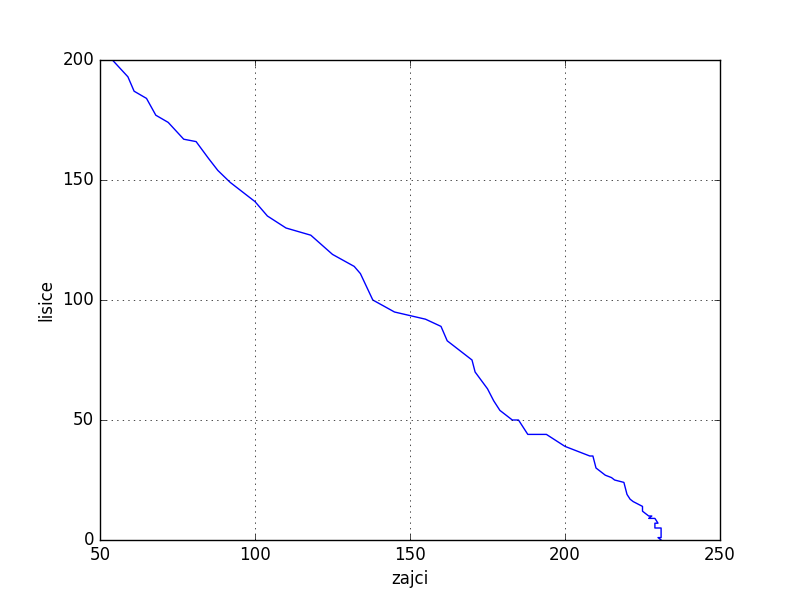
\includegraphics[scale=0.45]{slike/zajcki_lisice_fazni.png}
%\caption{second figure}
\end{minipage}
\caption{Rešitev populacije zajce in lisic po enačbi \ref{zajci-lisice-1}. Parametri: $L_0=50$, $Z_0=200$, $\alpha=5$, $\beta=4$, $\gamma=5$ $\delta=4$ ter $\Delta t=10^{-4}$.}
\end{figure}

\begin{figure}[h]
\begin{center}
\begin{minipage}{\textwidth}
\centering
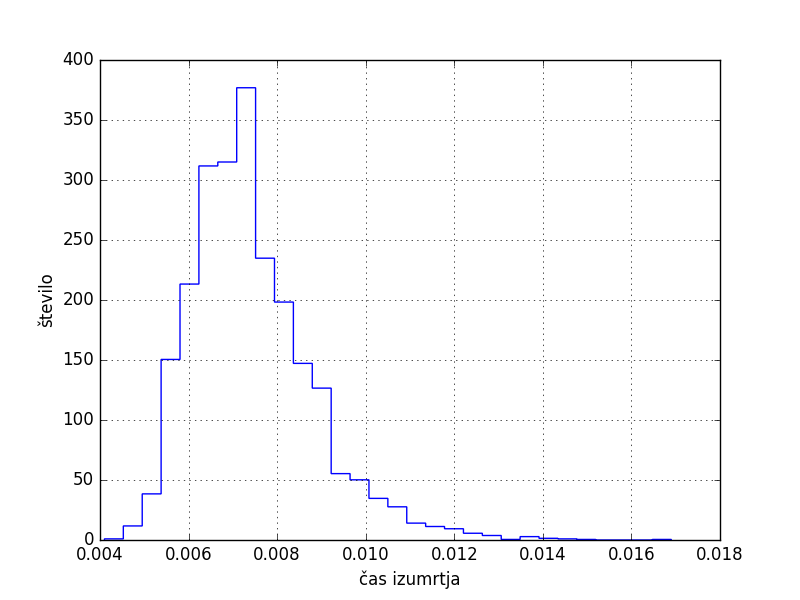
\includegraphics[scale=0.6]{slike/porazdelitev_zajcki_izumrli_cas.png}
%\caption{first figure}
\end{minipage}\hfill
\end{center}
\caption{Porazdelitev časov izumiranja zajcev. Parametri so enaki, kot v zgornjem primeru. Generiranih je bilo $5000$ časov. Povprečna vrednost je $0.00743$.}
\end{figure}





\end{document}
